\documentclass[a4paper,12pt,twoside]{book}
\usepackage[english]{babel}
\usepackage[utf8]{inputenc}
 \usepackage{hyperref}
\usepackage{graphics}
\usepackage{graphicx}
\usepackage{listings}
\usepackage{bera}
\usepackage{listings}
\usepackage{xcolor}
\pagestyle{headings}
 
\colorlet{punct}{red!60!black}
\definecolor{background}{HTML}{EEEEEE}
\definecolor{delim}{RGB}{20,105,176}
\colorlet{numb}{magenta!60!black} 
 
\lstdefinelanguage{json}{
    basicstyle=\normalfont\ttfamily,
    numbers=left,
    numberstyle=\scriptsize,
    stepnumber=1,
    numbersep=8pt,
    showstringspaces=false,
    breaklines=true,
    frame=lines,
    backgroundcolor=\color{background},
    literate=
     *{0}{{{\color{numb}0}}}{1}
      {1}{{{\color{numb}1}}}{1}
      {2}{{{\color{numb}2}}}{1}
      {3}{{{\color{numb}3}}}{1}
      {4}{{{\color{numb}4}}}{1}
      {5}{{{\color{numb}5}}}{1}
      {6}{{{\color{numb}6}}}{1}
      {7}{{{\color{numb}7}}}{1}
      {8}{{{\color{numb}8}}}{1}
      {9}{{{\color{numb}9}}}{1}
      {:}{{{\color{punct}{:}}}}{1}
      {,}{{{\color{punct}{,}}}}{1}
      {\{}{{{\color{delim}{\{}}}}{1}
      {\}}{{{\color{delim}{\}}}}}{1}
      {[}{{{\color{delim}{[}}}}{1}
      {]}{{{\color{delim}{]}}}}{1},
}
 
 
 \title{Data Wrangle OpenStreetMaps Data}
\date{February 3, 2015}
\author{Oleksii Renov}
        
\begin{document}
\maketitle

\section*{Choosing map area}
 
Choosing map area is very simple for me. I live in Kiev, Ukraine. So i hadn't got another choice. As the very first step I need minimum and maximum longitude and latitude. For this task I'd gone to \url{http://openstreetmap.org} in the search field I'd typed Kiev and choose the second link. I've the following web page in my browser.\par
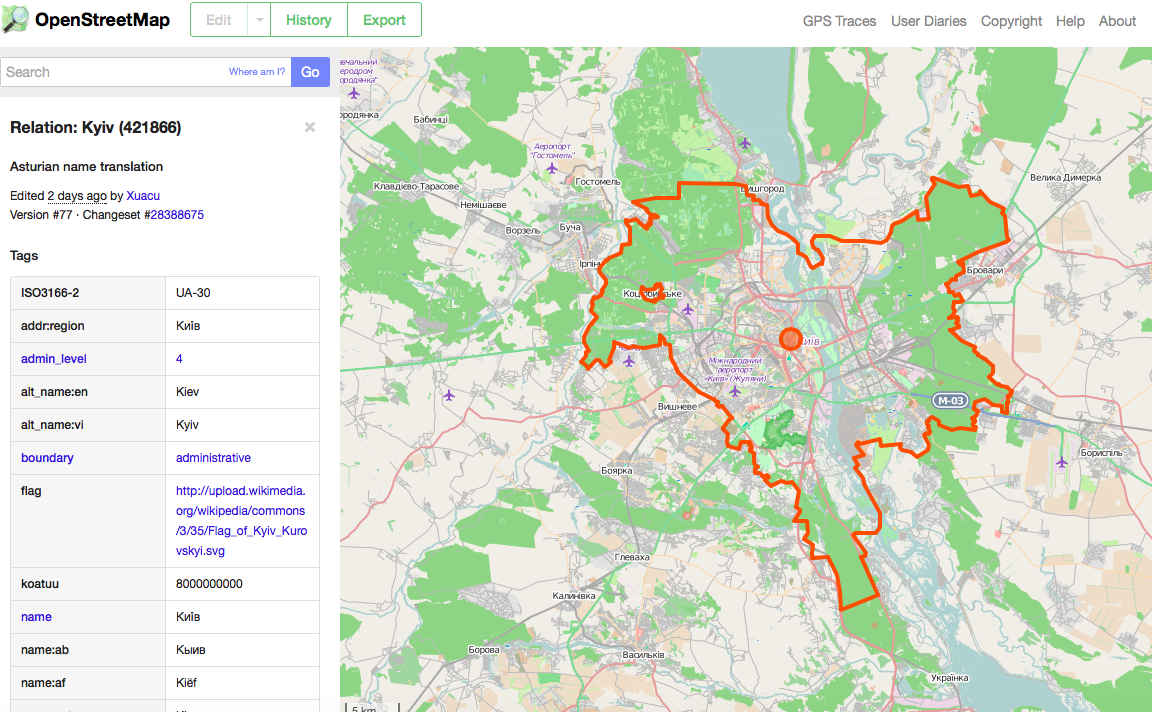
\includegraphics[scale=0.35]{keivinit.png}  
\par
I've done some zomming and choose next latitude and longitude parameters in my case:
\begin{itemize}
\item minimum latitude = 29.9048;
\item maximum latitude = 50.0986;
\item minimum longitude = 31.1600;
\item maximum longitude = 50.7052.
\end{itemize}
 
 Next step is to download my dataset. I've gone in \url{http://overpass-api.de/query_form.html}, where i can past some queries to download data what i need.\par

 My query is next:
 \begin{lstlisting}
(node(29.9048, 50.0986, 31.1600, 50.7052);<;);out;
\end{lstlisting}
Anyway there is exists numbers of variants loading data. One of them is simply go to this url \url{ http://overpass-api.de/api/map?bbox=29.9048,50.0986,31.1600,50.7052}. The xml file which I've already downloaded is very big, near 250mb. In my usual work i've chance working with xml, and files near 1mb is very hard to analyze. Let's move to processing this dataset.

\section*{Process Dataset}

As very first step, let's check what tags are in our dataset. Also would be helpful to check for attributes. Let's start from tags. 

\begin{lstlisting}[language=json,firstnumber=1]
{'bounds': 1,
 'member': 75124,
 'meta': 1,
 'nd': 1316743,
 'node': 1079619,
 'note': 1,
 'osm': 1,
 'relation': 5016,
 'tag': 417122,
 'way': 153102}
\end{lstlisting}
Next json is corresponded to tag attributes.
\begin{lstlisting}[language=json,firstnumber=1]
{'changeset': 1237737,
 'generator': 1,
 'id': 1237737,
 'k': 417122,
 'lat': 1079619,
 'lon': 1079619,
 'maxlat': 1,
 'maxlon': 1,
 'minlat': 1,
 'minlon': 1,
 'osm_base': 1,
 'ref': 1391867,
 'role': 75124,
 'timestamp': 1237737,
 'type': 75124,
 'uid': 1237737,
 'user': 1237737,
 'v': 417122,
 'version': 1237738}
\end{lstlisting}
First of all i would like to notice, that 'k' is key and 'v' is value. There are equal number of keys and values what is obvious. But it isn't clear what this keys are holding. I would like to explore more details and understand what keys and values have the most frequency in my dataset. In my opinion top 10 would be perfect for start.
\begin{lstlisting}[language=json,firstnumber=1]
{('surface', 9780),
 ('amenity', 9919),
 ('name:en', 10396),
 ('name:uk', 10646),
 ('name:ru', 12823),
 ('addr:street', 14084),
 ('name', 23862),
 ('addr:housenumber', 30646),
 ('highway', 67770),
 ('building', 73142)}
\end{lstlisting}
There are few nice things here. Due to Ukraine history we have official street name in ukrainian, unofficial russian and english names. For convinience I'm going to analyze here only international names. Let's check some values for key 'amenity'. For me it's very interesting.
\begin{lstlisting}[language=json,firstnumber=1]
 {('place_of_worship', 300),
 ('bench', 331),
 ('atm', 374),
 ('kindergarten', 419),
 ('fuel', 425),
 ('restaurant', 514),
 ('cafe', 520),
 ('school', 543),
 ('pharmacy', 566),
 ('bank', 770),
 ('parking', 1812)}
\end{lstlisting}
Let's try to analyze values, we've chosen three regular expressions to check text for lowercase, problem strings and others. Especially we would like to explore data with bad keys. 
\begin{lstlisting}[language=json,firstnumber=1]
{'lower': 258569,
'lower_colon': 163,
'other': 157676,
'problemchars': 714}
\end{lstlisting}
Let's take a loot at keys which values contain problem characters.
\begin{lstlisting}[language=json,firstnumber=1]
{'building:color': 2,
'contact:phone': 40,
'phone': 558,
'roof:colour': 19,
'wheelchair': 1}
\end{lstlisting}
There are exists more keys, but i want to point at not standartized phone numbers for this dataset. Let's look at them.
\begin{lstlisting}[language=json, firstnumber=1]
'+3-8-093-207-31-01, +3-8-067-838-47-64, +3-8-067-401-75-61'
 '+380 44 251-34-34',
 '+38(098)-109-5001',
 '+380 44 490 20 30',
 '+38 067 500 81 89',
\end{lstlisting}
Oh.. There are lots of phone numbers in different formats. I'm going to create one format for phone number for this dataset. It's can will be a list of phones even list can have only size equal to 1.\par
From wikipedia \url{http://en.wikipedia.org/wiki/Telephone_numbers_in_Ukraine} i've read that typical Ukrainian phone numbers is:
\begin{itemize}
\item +380 xx xxx-xx-xx (general phone numbers);
\end{itemize}
I've written script for this preprocessing, before converting data in JSON and loading data to MongoDB. Next little python script handle different data formats and standartize them.
\begin{lstlisting}[language=python, firstnumber=1]
def convertPhone(phone):
    # First step i'm going to remove all non number characters
    phone = re.sub('\D', '', phone)
    if len(phone) == 10:
        phone = "+38" + phone
    elif len(phone) == 7:
        phone = "+38044" + phone
    elif len(phone) == 12:
        phone = "+" + phone
    elif len(phone) == 11:
        phone = "+3" + phone
    elif len(phone) == 9:
        phone = "+380" + phone

    if len(phone) == 13:
        phone = phone[0:4] + ' ' + phone[4:6] + ' ' + phone[6:9] +
         '-' + phone[9:11] + '-' + phone[11:13]
    return phone
\end{lstlisting} 
Results of transformation:
\begin{itemize}
\item '+380(44)593-12-06' to '+380 44 593-12-06';
\item ' +380-44-599-60-82' to '+380 44 599-60-81';
\item '3317730' to '+380 44 331-77-30'.
\end{itemize}
Nice results.
\end{document}